% \documentclass[sigconf,authordraft]{acmart}
\documentclass[sigconf]{acmart}

\usepackage[utf8]{inputenc} % allow utf-8 input
%\usepackage[T1]{fontenc}    % use 8-bit T1 fonts
\usepackage{hyperref}       % hyperlinks
\usepackage{url}            % simple URL typesetting
\usepackage{booktabs}       % professional-quality tables
\usepackage{amsfonts}       % blackboard math symbols
\usepackage{nicefrac}       % compact symbols for 1/2, etc.
\usepackage{microtype}      % microtypography
\usepackage{lipsum}

\usepackage{amsmath,bm}     % bold
\newtheorem{theorem}{Theorem}[section]
\newtheorem{defn}[theorem]{Definition}  % definition
\newtheorem{cor}[theorem]{Corollary}    % corollary
\usepackage{enumerate}
\usepackage{subfigure}
\usepackage{listings}  % code block
%\usepackage{inconsolata}  % consola
% \usepackage{fontspec}  % specify font, only for xelatex
% \newfontfamily{\ttconsolas}{Consolas}
\usepackage{enumitem}

\AtBeginDocument{%
  \providecommand\BibTeX{{%
    \normalfont B\kern-0.5em{\scshape i\kern-0.25em b}\kern-0.8em\TeX}}}

\setcopyright{acmcopyright}
\copyrightyear{2020}
\acmYear{2020}
\acmDOI{xx.xxxx/xxxxxxx.xxxxxxx}

\acmConference[SIGMOD '20]{SIGMOD '20: ACM International Conference on Management of Data}{June 14 - 19, 2020}{Portland, Oregon}
\acmBooktitle{SIGMOD '20: ACM International Conference on Management of Data, June 14 - 19, 2020, Portland, Oregon, USA}
\acmPrice{15.00}
\acmISBN{978-x-xxxx-xxxx-x/xx/xx}

\author{Leave Authors Anonymous}
\affiliation{%
  \institution{}
  \streetaddress{}
  \city{}
  \country{}}
\email{}

\begin{document}

\title{Querying Video Interactions}

% \renewcommand{\shortauthors}{, et al.}

\begin{abstract}
As deep neural nets enabled sophisticated information extraction out of images, including video frames, there has been recent interest in techniques and algorithms to allow interactive declarative query processing on objects and their interactive constraints on video feeds. 
In this demo, we present a system for declarative querying on real-time video streams involving objects and their interactions. The system utilizes a sequence of inexpensive and less accurate models (filters), called Progressive Filters (PF), to detect the presence of the query specified objects on frames. 
Since selectivities may vary as the video evolves, the system deploys a dynamic statistical test to determine when to trigger the re-optimization of the filters. 
In the end, the system presents a filtering approach, called Interaction Sheave (IS), which utilizes learned spatial information about objects and interactions to effectively prune frames that are not likely to contain interaction.
We demonstrate that this system can efficiently identify frames in a streaming video in which an object is interacting with another in a specific way, increasing the frame processing rate dramatically and speed up query processing by at least two orders of magnitude depending on the query. 
\end{abstract}

\maketitle

\keywords{First keyword, Second keyword and More }

\section{Introduction}

Recent advances in computer vision - in the form of deep neural networks - have made it possible to query increasing volumes of video data with high accuracy. However, deep neural network inference is computationally expensive at scale. Although some have proposed systems for accelerating deep neural network queries on videos, there are still many limitations to apply them to real-world scenarios. 

To understand the visual world, a machine must not only recognize individual object instances but also how they interact. Most of the state-of-the-art video query processing models focus on the queries about the number of classified objects and their location relationships \cite{kang2017noscope, kang2018blazeit, Xarchakos2019, koudas2020video}. Semantic information, such as human-object interaction information, is often ignored. Fortunately, several state-of-the-art algorithms in the fields of object detection, object classification and object tracking in images and videos are proposed \cite{girshick2014rich, gkioxari2018detecting, krizhevsky2012imagenet, simonyan2014very}. They provide the ability to classify objects and detect object locations in a frame as well as track objects from frame to frame with adequate accuracy. 

\begin{figure}[H]
  \centering
   \subfigure{
    \label{fig:baseball} 
    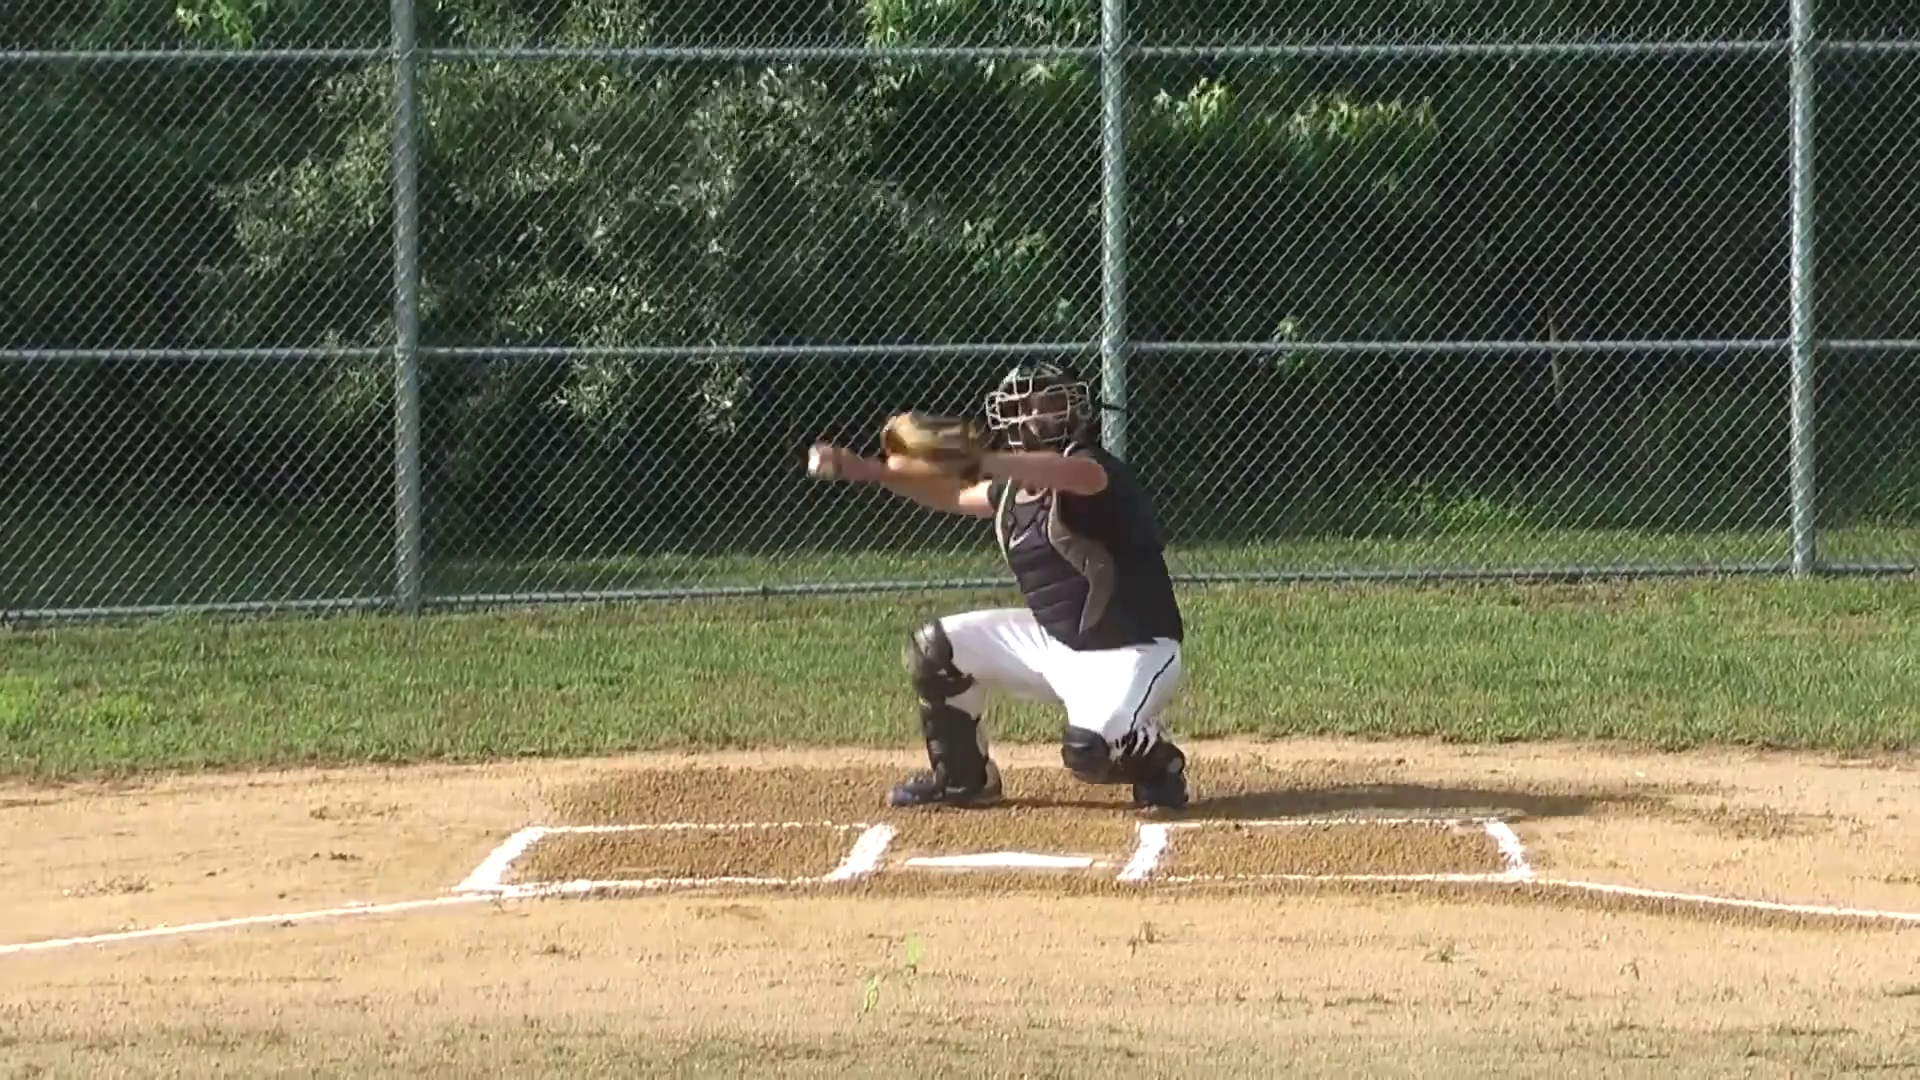
\includegraphics[width=0.25\textwidth]{graphs/baseball.jpg}
  }
%  \hspace{.1in} 
  \subfigure{
    \label{fig:tennis} 
    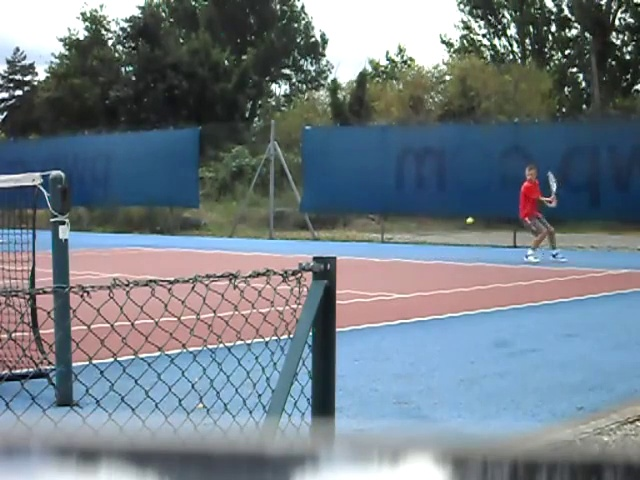
\includegraphics[width=0.19\textwidth]{graphs/tennis.jpg}
  }
  \caption{Examples of interactions.}
  \label{fig:examples} %% label for entire figure
\end{figure}

\begin{figure*}[h]
\centering
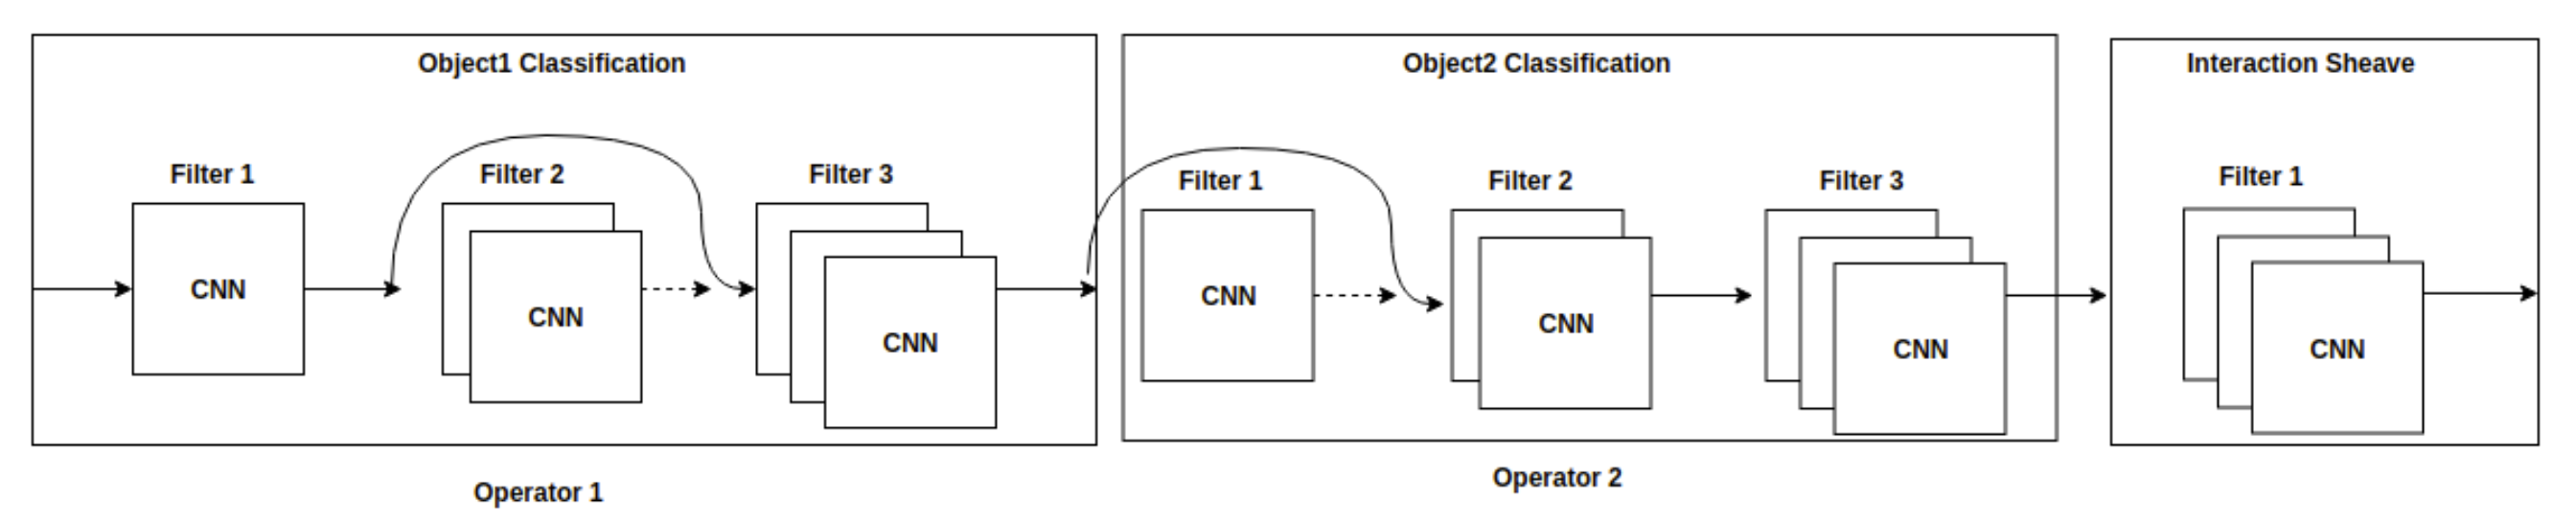
\includegraphics[width=1\textwidth]{graphs/architecture.png}
\caption{Example of the overall architecture.}
\label{fig:architecture}
\end{figure*}

Video monitoring and surveillance applications are of particular interest in our system, where a static camera records activity in its receptive range. Several recent works \cite{kang2017noscope, kang2018blazeit, koudas2020video, Xarchakos2019} focus in these domains, to provide declarative queries based on streaming video feeds. Our work complements and enhances this research line with a focus on efficiently executing interaction query primitives, i.e., capturing interactions among query objects. 
Many interesting queries become possible when we can query object interactions. For example, automatically detecting frames in which a human holds a gun or a human breaks a window would be of great interest in surveillance and security applications. 
Figure \ref{fig:examples} presents examples of interactions between a human and a ball (videos from Kinetics Dataset \cite{carreira2019short}). The corresponding query in SQL for the interaction at the frame of Figure \ref{fig:baseball} would be:
\begin{lstlisting}[language = SQL, keywordstyle=\color{blue!100}, 
    commentstyle=\color{red!50!green!50!blue!50}, 
    rulesepcolor=\color{red!20!green!20!blue!20}, 
    basicstyle=\footnotesize\ttfamily,
    breaklines=true,]
SELECT cameraID, frameID, C1 (F1 (HumanBox1)) AS HumanType1, C2 (F2 (Ballbox1)) AS BallType1,
FROM (PROCESS inputVideo PRODUCE cameraID, frameID, HumanBox1 USING HumanDetector, BallBox1 USING BallDetector) 
WHERE HumanType1 = human AND BallType1 = baseball AND INTERACTION(HumanType1, BallType1) = THROW
\end{lstlisting}
The query employs two classifiers ($C_i$) to detect a \emph{human} and a \emph{baseball}, using features $F_i$ extracted from the frame and checking whether the objects, once identified, are related via a THROW interaction. Obviously, from an execution perspective, it makes sense to invoke the INTERACTION predicate once the operands have been identified on the frame. We seek to automatically identify frames in a video stream where query objects interact in a specific way. 
The main emphasis of this system is, given a query involving objects and their interaction on a video stream, to propose algorithms to efficiently determine which frames are expected to be part of the query answer and filter out all irrelevant frames. Therefore, we try to increase the frame processing rate as frames that are considered irrelevant will not be processed further but skipped quickly. Even without filtering, the application of deep neural networks for object and interaction detection entails false positives/negatives. We will also show the effect that filtering has on the false positive/negative rate of the techniques on this demo. 
 
To overcome these challenges, we present a set of algorithms that dramatically increase the frame processing rate when executing the query while maintaining high accuracy. In particular, the set of algorithms are as follows. 
\begin{itemize}[itemsep=0pt, topsep=0pt, leftmargin=0pt, itemindent=20pt]
\item \textbf{Progressive Filters.} 
Progressive filters are a set of filters of increasing cost (i.e., an increasing number of network layers). For a particular object type, progressive filters use the selectivity of the filters to derive the optimal filter sequence. The filters should be applied to minimize the total cost of processing the video stream. 
\item \textbf{Triggering Re-optimization.} 
Since we observe that the statistical properties of certain types of objects vary over time on a video stream, we adopt a dynamic version of the Kolmogorov-Smirnoff test \cite{massey1951kolmogorov} that can trigger progressive filters algorithm when the statistical properties of the filter selectivity change. We are effectively adjusting the filter sequence, in anticipation of stable (predictable) object statistics, until the next re-optimization. Such a strategy can improve accuracy while maintaining a high frame processing rate. 
\item \textbf{Interaction Sheave.} 
Interaction sheave is a filtering mechanism for object interaction queries. It can inspect the spatial location of objects on frames and filter out frames that although contain objects relevant to the query but not promising to encompass the suitable interaction among the query objects.
\end{itemize}

In this demonstration, we showcase our Querying Video Interactions system, which is capable of handling a wide range of interaction queries. Section \ref{sec:architecture} presents the architecture of our system. Section \ref{sec:demonstration} presents a description of this demonstration. Section \ref{sec:conclusion} concludes this demo and discusses future work in this area. 


\section{System Architecture}
\label{sec:architecture}

Deep learning filters is an extensible module that implements our proposed filter predicates, which encompasses popular recent deep learning algorithms for object detection, texture/shape extraction, as well as algorithms for precise object localization on a video frame. It enables count estimation of objects of a specific class and location estimation of the objects in the frames. 
These algorithms are embedded in the parsed query representation and relayed to the query execution engine. The execution module utilizes popular deep learning frameworks to execute the query with the assistance of available GPUs. Frames that pass the filters instantiated in the query are subsequently checked with deep learning predicates and then routed to the front end for display.

An example of the architecture of our proposed filter technologies is shown in Figure \ref{fig:architecture}. There are two operators, each consisting of a number of filters. The application of progressive filters for operator 1 determined that filters 1 and 3 are currently in use. Similarly, for operator two, filters 2 and 3 are in use. Frames that successfully pass the operators with a positive determination\footnote{Take the first operator as an example, a frame may get a positive determination by filter 1; in that case, there is no need for further processing by other filters in this operator. Filter 3 (a more accurate and expensive model in this example) is involved only if Filter 1 is unable to make a positive or negative determination for the frame.} that they contain the objects of interest, are tested by the Interaction Sheave. 
Our focus in this work is how to order filters within an object detection operator effectively. Typically, a query will check for the presence of more than one object (as in the case of the sample SQL query presented). 
The progressive filters can derive the least cost sequence of filters given the current selectivities of query objects, avoiding costly object detection and localization operations, and minimizes the cost per frame for object detection. 
For the filters employed, we can maintain their selectivities up to date by observing the result of each frame tested by the filter. For the filters that are not part of the optimal solution, we periodically (every few seconds) route a frame from the input sequence through them and obtain a selectivity estimate to trigger re-optimization. 
For frames that pass through the filter sequences determined by progressive filters for each object specified by the query, we have confidence that they contain the required objects. These models will derive a bounding box that encloses the location of each object as specified by the query on the frame. We then test the frame whether it relates the objects via the query specified interaction. 

\subsection{Progressive Filters}
\label{sec:progressivefilters}

We test whether the objects of the class specified by the query are present in the frame before we check a frame for a query specified interaction among objects. Such a test can take place by involving state of the art object classification or detection models \cite{girshick2015fast, simonyan2014very}. Although such models have high accuracy, they impose large overheads in terms of processing time per frame. Prior work \cite{kang2017noscope, Xarchakos2019} has utilized inexpensive filters that are trained apriori or on-demand to reduce processing overheads at the expense of accuracy. 
They are typically trained to achieve specific false positive and false negative rates, while relaying any other decision to high accuracy (but more expensive) model. Such a filter quickly determines whether a frame contains an object of a specific type or not. The premise of such filters is that a significant fraction of frames are not relevant to the query and can be dropped quickly. Moreover, relevant frames can be positively decided by the inexpensive filter, and only tough cases will involve an expensive model. 
% If the filter is uncertain about making such determination, it invokes a high accuracy filter to process the frame further. 

We observe that the pruning efficiency of such a filtering approach can be improved by deploying a series of inexpensive filters that progressively have higher accuracy and higher cost. Therefore, we realize an object detection operator as a sequence of filters. Assessing the selectivity for each of the filter predicates, we propose a practical algorithm that derives the optimal set of filter predicates for an object type to deploy. Thus, we address the inter-operator scheduling of filters to minimize detection cost. Assuming the future statistical characteristics of the video stream remain the same, the filtering combination will reduce the cost (alternatively maximize frame processing rate) to process the video stream and determine frames that contain the specific object type.

\subsection{Triggering Re-optimization}
\label{sec:triggering}

Since one cannot expect the distribution of objects on video frames over time to remain the same, we propose an algorithm to assess incrementally when the statistical properties of the underlying object distribution change. When such properties change, we trigger re-optimization, deriving a new optimal filter sequence to deploy. The basic idea behind our proposal is to treat the selectivity of filters as a statistical population and employ a dynamic version of the popular Kolmogorov-Smirnov test \cite{massey1951kolmogorov}. In that way, we monitor the underlying distribution of objects relevant to the query between two epochs and trigger re-optimization when the statistical properties change.

\subsection{Interaction Sheave}
\label{sec:sheave}

In order to address our ultimate objective, each frame that contains the specified objects has to be processed by a deep learning model that determines the type of interaction between objects \cite{gkioxari2018detecting, kolesnikov2019detecting, ma2017grounded, ulutan2018actor}. 
%These models determine if the frame is relevant to the query. 
However, such object interaction models impose their own overheads per frame. To improve the frame processing rate even further, we develop a filtering mechanism for object interactions. The basic observation is that the interaction (e.g., human throwing a baseball) typically takes place at a specific spatial region of the frame involving the first object (i.e., the human). For each type of interaction, we could propose a model to identify such regions. Only when the second object is located within a spatial region relative to the first object, the frame is relayed to an expensive object interaction model for further processing. Thus, by processing the objects spatially, we obtain a filtering mechanism for interaction. 
Our final proposal combines these three techniques delivering an effective framework to process object interaction queries, efficiently improving the frame processing rate in a video stream dramatically.


\section{Demonstration Setup}
\label{sec:demonstration}

\begin{figure*}[h]
\centering
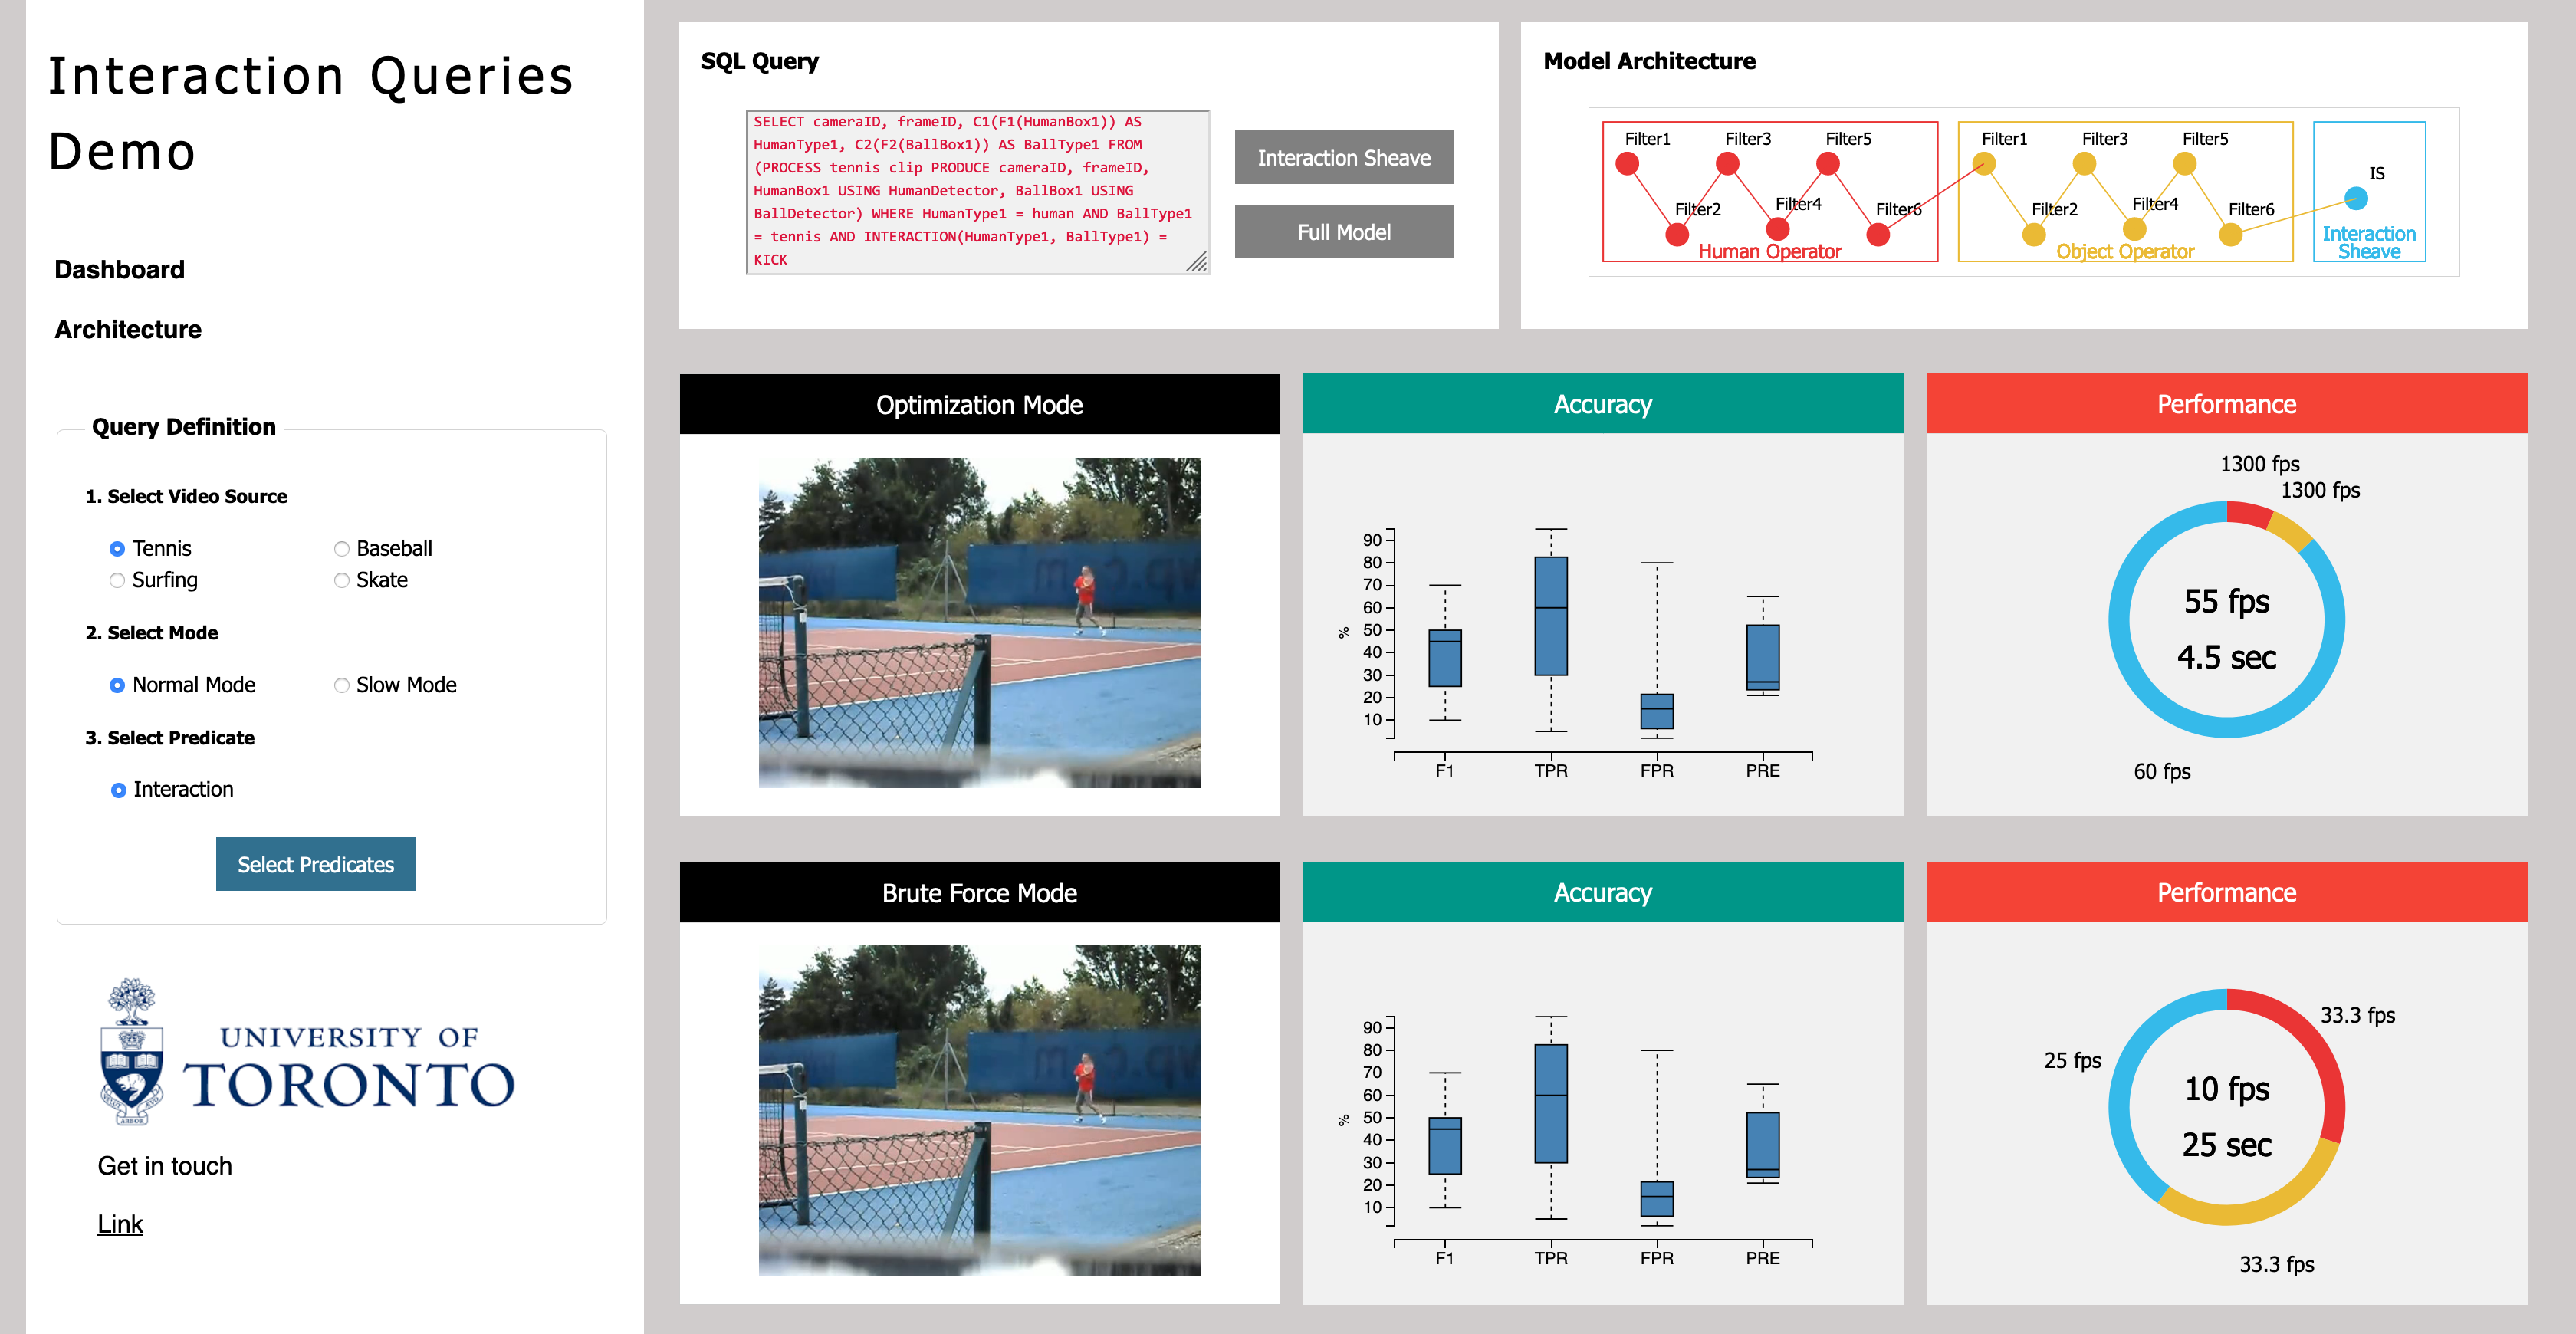
\includegraphics[width=0.99\textwidth]{graphs/demo.png}
\caption{Video Stream Interaction Queries demo.}
\label{fig:frontend}
\end{figure*}

\begin{figure*}[t]
\centering
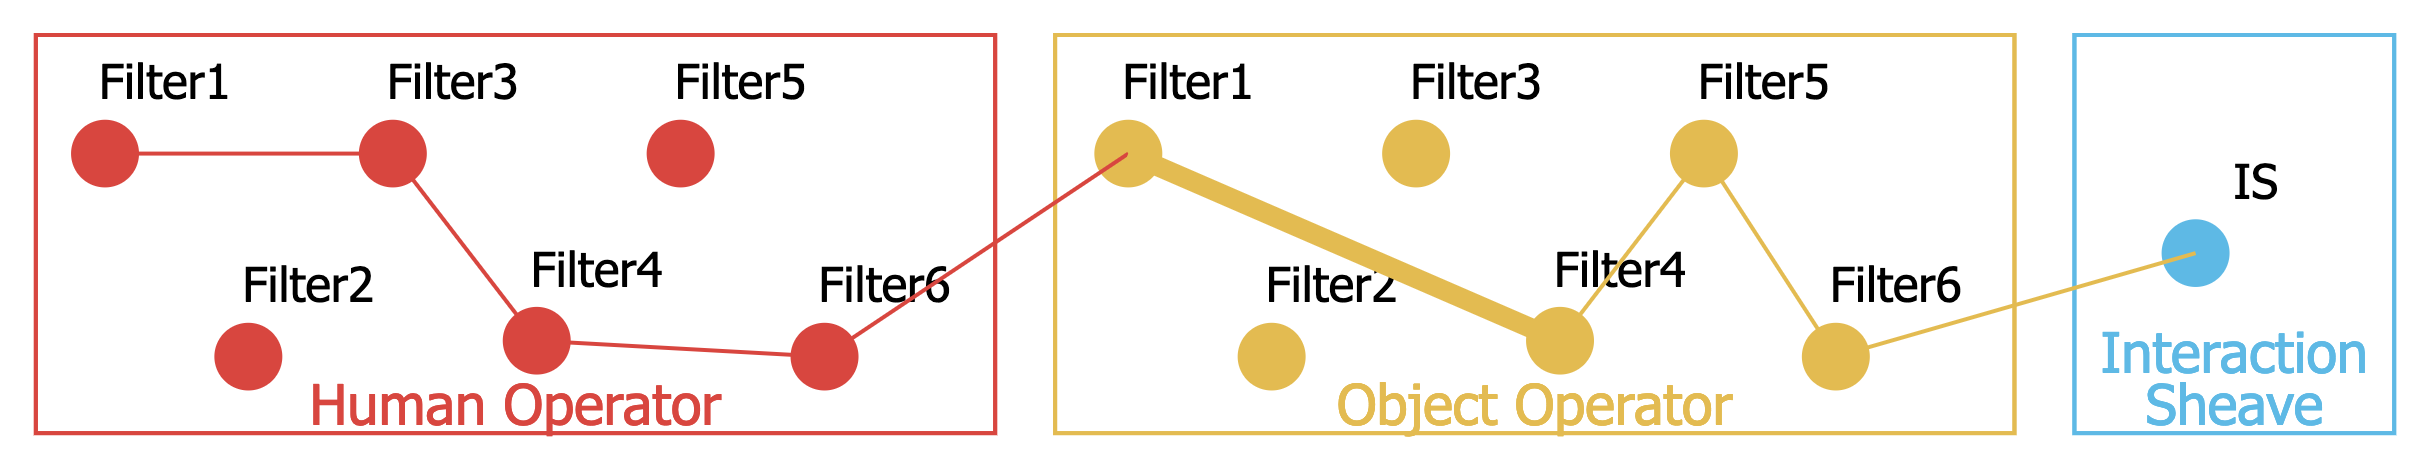
\includegraphics[width=0.7\textwidth]{graphs/filters.png}
\caption{Filters ordering module.}
\label{fig:filters}
\end{figure*}

This demo simulates the interaction querying process and provides various knobs for video source selection, performance monitoring and query results display and comparisons. It currently incorporates the layout of \cite{Xarchakos2019} with few new features. Our layout, will allow users to express human object interaction queries and compare the time and accuracy performance of our approach with the full model's performance \cite{gkioxari2018detecting}. 

Figure \ref{fig:frontend} presents the current state of the front end. 
SQL queries are defined through query definition which is shown in the left sidebar (Area A) and enhanced with UDFs to manipulate video object primitives.  
The Demo provides four video clips for interaction querying. Each video clip corresponds to a specific predicate. For the baseball video clip, for instance, the predicate will be \emph{human THROW baseball}. 
The Demo also provides two modes - normal and slow mode. The normal mode shows the real video processing speed of our system, while it may run too fast to show the results of interaction detection. For better implementation, it also provides a slow mode to show the resulting video which is slower than the real processing speed. 

The generated SQL queries, which are shown on the upper left center (Area B), are dispatched to the back end which is responsible for parsing the query and incorporating the supported querying predicates and progressive filters. 
It currently incorporates our proposed algorithms for filtering frames (based on humans, objects classes and interaction), allowing to express semantically meaningful video frame queries in an interactive fashion. 
The impact of progressive filters will be analyzed based on the total query processing time (when compared to a query that does not make use of the progressive filters but instead executes the query in a brute force manner \cite{gkioxari2018detecting} as well as the resulting frame processing rate. 

The filters' ordering per batch is presented on the upper right corner (Area C). It will be updated at the end of each batch. The three boxes with different colors represent different operators and a node in a box represents a filter in the operator. 
As introduced in section \ref{sec:progressivefilters}, the application of algorithm progressive filters may employ a subset of filters. The links represent the ordering of filters that are used for the current batch. 
As introduced in section \ref{sec:triggering}, for the filters that are not part of the optimal solution, we periodically route a frame from the input sequence through them and obtain a selectivity estimate as well. The links will be bold if they have been changed from the previous batch to the current. 
Figure \ref{fig:filters} presents the filters ordering module. The red box and nodes represent human operators, whose Filter 1, 3, 4 and 6 are used. Similarly, the yellow and blue represent the object operator and interaction sheave respectively. 

By clicking on the Optimization button, our approach will be invoked, while by clicking the Brute Force button, state of the art object detectors \cite{8237584He2017} and action recognition \cite{gkioxari2018detecting} models will evaluate the respective input video. 
The videos of both our approach and full model's approach will produce bounding boxes for humans and objects which participate in an interaction. Additionally, a heat-map on frames where a specific interaction exists between the human and the object. Areas D and G present the actual query results for our proposed techniques and brute force respectively. 
F1 score and precision/recall results are reported in Areas E (for our algorithms) and H (for brute force), complemented with detailed performance numbers (response times and frame rates) in areas F and I respectively. 

\section{Conclusion and Future Work}
\label{sec:conclusion}

This demo showcases our Querying Video Interactions system.
The system we proposed constitutes a robust approach to process video streams for query specified object interactions, achieving a very high frame processing rate. 
This work sheds light on declarative query process for video streams. New query types involving spatial and temporal predicates require intensive future research. 
The extension of the filters for crowd counting and estimation scenarios is also necessary. 


\bibliographystyle{ACM-Reference-Format}
\bibliography{references}

\end{document}
\endinput
